%%%%%%%%%%%%%%%%%%%%%%%%%%%%%%%%%%%%%%%%%%%%%%%%%%%%%%%%%%%%%%%%%%%%%%%%%%%%%%%
% Copyright 2019
% Liturgy of St. John Chrysostom for regular Sundays
% Simple traditional Arabic chants through to the Trisagion,
% and then switching to more choral for the remainder of the service.
%%%%%%%%%%%%%%%%%%%%%%%%%%%%%%%%%%%%%%%%%%%%%%%%%%%%%%%%%%%%%%%%%%%%%%%%%%%%%%%

\documentclass[twoside, letterpaper, 12pt]{report}
\usepackage{orthodoxservicebook}
\title{Divine Liturgy\\
As celebrated on most Sundays which are not Feast days}

\author{St. Katherine Orthodox Church}
\date{}% Remove date
\titlepic{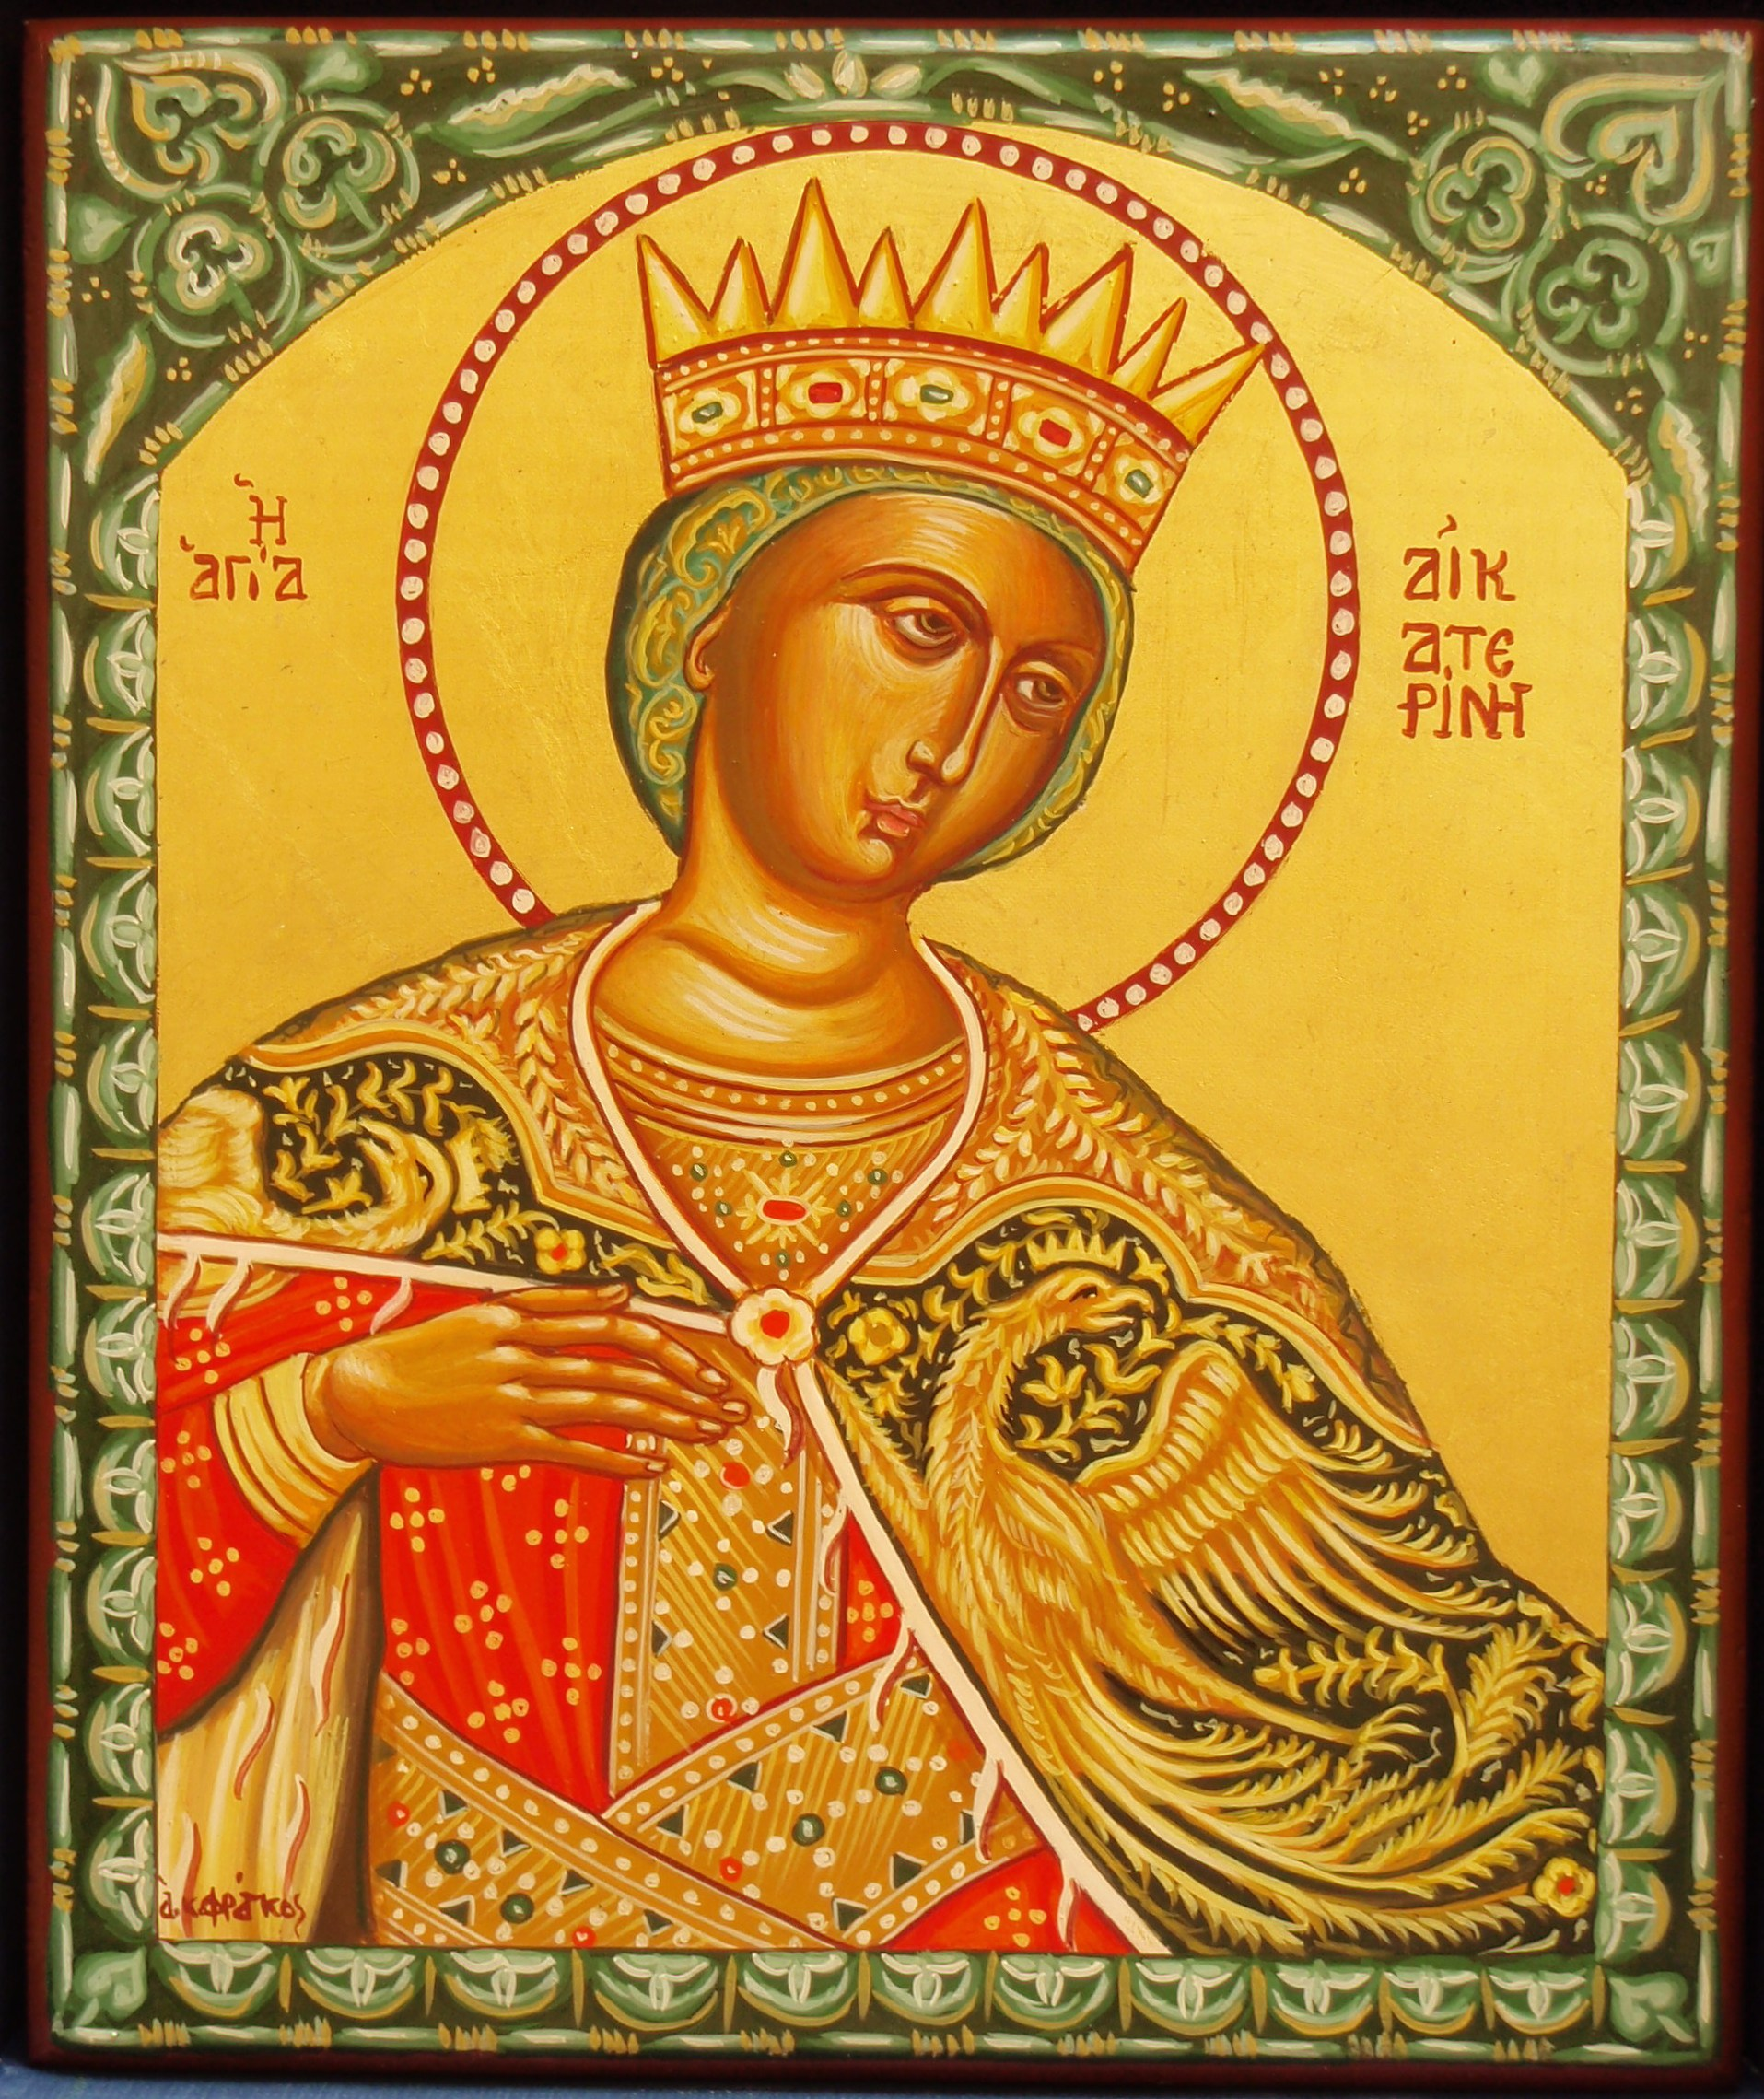
\includegraphics[width=0.5\textwidth]{Katherine1.jpg}}

\begin{document}
\maketitle
\pagestyle{empty}
\instruction{This page intentionally left blank}
\cleardoublepage
\pagestyle{plain}

\chapter*{Divine Liturgy}

\centeredsection{Preparation and Opening Dialogue}

\begin{priest}
\item O heavenly King, Comforter, the Spirit of truth,
who art everywhere present and fillest all things,
the Treasury of good things and Giver of life:
Come and abide in us and cleanse us from every stain and save our souls,
O Good One.
\item Glory to God in the highest, and on earth peace, good will among men \instruction{2x}
\item O Lord, Thou shalt open my lips, and my mouth shall declare Thy praise.
\end{priest}

\deaconline{It is time for the Lord to act. Bless, father.}
\priestline{Blessed is our God, always, now and ever, and unto ages of ages.}
\deaconline{Amen. Pray for me, father.}
\priestline{The Lord direct thy steps unto every good work.}
\deaconline{Remember me, holy father.}
\priestline{The Lord God remember thee in His kingdom, always, now and ever, and unto ages of ages.}
\begin{deacon}
\item Amen.
\item O Lord, thou shalt open my lips, and my mouth shall declare Thy praise.
\item Bless, father
\end{deacon}

\instruction{This is proclaimed loudly, and signifies that preparations are complete,
  and the service is now beginning}
\priestline{Blessed is the kingdom of the Father and of the Son and of the Holy Spirit,
   now and ever and unto ages of ages.}

\lilypondfile{./Z-Responses/Kazan/Amen.ly}

% Want to ensure this pretty much starts on a new page.
\needspace{20\baselineskip}
\centeredsection{The Litany of Peace}

\deaconline{In peace, let us pray to the Lord.}
\instruction{Repeat these responses until the last petition.}
\lilypondfile{./Z-Responses/Kazan/LordHaveMercy-A.ly}

\deaconline{For the peace from above and the salvation of our souls, let us pray to the Lord.}
\lilypondfile{./Z-Responses/Kazan/LordHaveMercy-B.ly}

\deaconline{For the peace of the whole world, the good estate of the holy churches of God
  and the union of all men, plet us pray to the Lord.}
\lilypondfile{./Z-Responses/Kazan/LordHaveMercy-C.ly}

\begin{deacon}
\item For this Holy House, and for those who with faith, reverence,
  and fear of God, enter therein,
  let us pray to the Lord.
\item For our father and Metropolitan N., (for our Archbishop N. or Bishop N.),
  for the venerable Priesthood, the Diaconate in Christ, for all the clergy and the people,
  let us pray to the Lord.
\item For the President of the United States, for all civil authorities,
  and for our Armed Forces everywhere, let us pray to the Lord.
\item For this city, and for every city and land, and for the faithful who dwell therein,
  let us pray to the Lord.
\item For healthful seasons, for abundance of the fruits of the earth, and for peaceful times,
  let us pray to the Lord.
\item For travelers by sea, by land, and by air; for the sick and the suffering;
  for captives and their salvation,
  let us pray to the Lord.
\item For our deliverance from all tribulation, wrath, danger, and necessity,
  let us pray to the Lord.
\item Help us; save us; have mercy on us; and keep us, O God, by Thy grace.
\end{deacon}
\lilypondfile{./Z-Responses/Kazan/LordHaveMercy-Z.ly}

\deaconline{Calling to remembrance our all-holy, immaculate, most blessed and glorious Lady the Theotokos\\
  \instruction{(Recited quietly as the petitioner continues)}\\
  \lilypondfile[staffsize=15]{./Z-Responses/Kazan/MostHolyTheotokosSaveUs.ly}\\
  and ever-virgin Mary, with all the Saints: let us commend ourselves and each other,
  and all our life unto Christ our God.
}

\lilypondfile{./Z-Responses/Kazan/ToTheeOLord.ly}

\priestline{For unto Thee are due all glory, honor, and worship:
  to the Father, and to the Son, and to the Holy Spirit; now and ever and unto ages of ages.}
\lilypondfile{./Z-Responses/Kazan/Amen.ly}

\centeredsection{The First Antiphon}
\lilypondfile{./Liturgy/B-FirstAntiphon/TheFirstAntiphon-Tone2SimpleByzChant-Music.ly}


\centeredsection{The Little Litany}
\deaconline{Again and again, in peace, let us pray to the Lord.}
\lilypondfile{./Z-Responses/Kazan/LordHaveMercy-A.ly}

\deaconline{Help us, save us, have mercy on us; and keep us, O God, by Thy grace.}
\lilypondfile{./Z-Responses/Kazan/LordHaveMercy-B.ly}

\needspace{5\baselineskip}
\deaconline{Calling to remembrance our all-holy, immaculate, most blessed and glorious Lady the Theotokos\\
  \instruction{(Recited quietly as the petitioner continues)}\\
  \lilypondfile[staffsize=15]{./Z-Responses/Kazan/MostHolyTheotokosSaveUs.ly}\\
  and ever-virgin Mary, with all the Saints: let us commend ourselves and each other,
  and all our life unto Christ our God.
}

\lilypondfile{./Z-Responses/Kazan/ToTheeOLord.ly}

\priestline{For Thine is the might, and Thine is the kingdom and the power and the glory
  of the Father and of the Son and of the Holy Spirit, now and ever, and unto ages of ages.}

\lilypondfile{./Z-Responses/Kazan/Amen.ly}

\centeredsection{The Second Antiphon}
\lilypondfile{./Liturgy/C-SecondAntiphon/TheSecondAntiphon-Tone2SimpleByzChant-Music.ly}
\needspace{10\baselineskip}
\lilypondfile{./Liturgy/C-SecondAntiphon/GNE-OnlyBegottenSon-Tone2SimpleByzChant-Music.ly}

\centeredsection{The Little Litany}
\deaconline{Again and again, in peace, let us pray to the Lord.}
\lilypondfile{./Z-Responses/Kazan/LordHaveMercy-A.ly}

\deaconline{Help us, save us, have mercy on us; and keep us, O God, by Thy grace.}
\lilypondfile{./Z-Responses/Kazan/LordHaveMercy-B.ly}

\needspace{5\baselineskip}
\deaconline{Calling to remembrance our all-holy, immaculate, most blessed and glorious Lady the Theotokos\\
  \instruction{(Recited quietly as the petitioner continues)}\\
  \lilypondfile[staffsize=15]{./Z-Responses/Kazan/MostHolyTheotokosSaveUs.ly}\\
  and ever-virgin Mary, with all the Saints: let us commend ourselves and each other,
  and all our life unto Christ our God.
}

\lilypondfile{./Z-Responses/Kazan/ToTheeOLord.ly}

\priestline{For Thou art a good God and lovest mankind,
  and unto thee we ascribe glory to the Father and to the Son and to the Holy Spirit,
  now and ever, and unto ages of ages.}
\lilypondfile{./Z-Responses/Kazan/Amen.ly}

\centeredsection{Apolytikion}
\instruction{Sing the Apolytikion appointed for the day as the 3rd antiphon before the entrance.}

\centeredsection{The Little Entrance}
\lilypondfile{./Liturgy/E-LittleEntrance/TheLittleEntrance-Tone2SimpleByzChant-Music.ly}

\centeredsection{Apolytikia}
\instruction{Again, sing the Apolytikia in the order appointed for the day.}
\clearpage
\begin{variables}{timberwolf}
\needspace{20\baselineskip}
\centeredsubsection{Tone - 1}
\needspace{20\baselineskip}
\lilypondfile{./Octoechos/ResurrectionalApolytikion-Tone1-Kazan-Music.ly}
\needspace{20\baselineskip}
\centeredsubsection{Tone - 2}
\lilypondfile{./Octoechos/ResurrectionalApolytikion-Tone2-Kazan-Music.ly}
\needspace{20\baselineskip}
\centeredsubsection{Tone - 3}
\lilypondfile{./Octoechos/ResurrectionalApolytikion-Tone3-Kazan-Music.ly}
\needspace{20\baselineskip}
\centeredsubsection{Tone - 4}
\lilypondfile{./Octoechos/ResurrectionalApolytikion-Tone4-Kazan-Music.ly}
\needspace{20\baselineskip}
\centeredsubsection{Tone - 5}
\lilypondfile{./Octoechos/ResurrectionalApolytikion-Tone5-Kazan-Music.ly}
\needspace{20\baselineskip}
\centeredsubsection{Tone - 6}
\lilypondfile{./Octoechos/ResurrectionalApolytikion-Tone6-Kazan-Music.ly}
\needspace{20\baselineskip}
\centeredsubsection{Tone - 7}
\lilypondfile{./Octoechos/ResurrectionalApolytikion-Tone7-Kazan-Music.ly}
\needspace{20\baselineskip}
\centeredsubsection{Tone - 8}
\lilypondfile{./Octoechos/ResurrectionalApolytikion-Tone8-Kazan-Music.ly}
\end{variables}

\centeredsubsection{Apolytikion for Great-martyr Katherine the all-wise of Alexandria}
\instruction{On usual Sundays, one of the Apolytikia is that of the patron saint of the community}
\lilypondfile{./Menaion/11-25-StKatherine/Katherine-Trop_Tone5ByzChant-Music.ly}

\centeredsection{Kontakion}
\instruction{Sing the Kontakion in the order appointed for the day. }

\centeredsubsection{Kontakion to the Theotokos for Usual Sundays}
\instruction{On usual Sundays, the Kontakion is the `O Protection of Christians' hymn to the Theotokos}
\lilypondfile{./Liturgy/H-Kontakion/OProtectionOfChristians_Tone2ByzChant-Music.ly}

\centeredsection{The Prayer of the Thrice-Holy Hymn}
\deaconline{Let us pray to the Lord}
\lilypondfile{./Z-Responses/Kazan/LordHaveMercy-A.ly}

\priestline{For holy art Thou, O our God, and unto Thee we ascribe glory
  to the Father and to the Son and to the Holy Spirit, now and ever...}
\deaconline{... and unto ages of ages.}

\lilypondfile{./Z-Responses/Obikhod/Amen.ly}

\centeredsection{The Thrice-Holy Hymn}
\instruction{This may be replaced by the Baptismal or Hymn for the Cross as prescribed}
\vspace{12pt}
\lilypondfile{./Liturgy/I-ThriceHolyHymn/Trisagion_Arabic_a.ly}
\deaconline{With Strength.}
\lilypondfile{./Liturgy/I-ThriceHolyHymn/Trisagion_Arabic_b.ly}

\cleardoublepage
\begin{variables}{timberwolf}
\centeredsection{Anti-Trisagion\\Baptismal Hymn}
\instruction{Sung on certain days instead of the Thrice Holy Hymn}
\vspace{5pt}
\lilypondfile{./Liturgy/I-ThriceHolyHymn/AsManyAsHaveBeen-ByzPlain-a_Music.ly}
\deaconline{With Strength.}
\lilypondfile{./Liturgy/I-ThriceHolyHymn/AsManyAsHaveBeen-ByzPlain-b_Music.ly}
\clearpage
\centeredsection{Anti-Trisagion\\Before Thy Cross}
\instruction{Sung on certain days instead of the Thrice Holy Hymn}
\vspace{5pt}
\lilypondfile{./Liturgy/I-ThriceHolyHymn/BeforeThyCross-Traditional_Music.ly}
\end{variables}


\centeredsection{The Readings from the New Testament}

\instruction{The appointed reader prepares to read the prokeimenon, facing the Royal Doors}

\deaconline{Let us attend}

\readerline{\instruction{Announces the prokeimenon of the epistle}}

\deaconline{Wisdom}

\readerline{\instruction{Announces the title of the epistle}}

\deaconline{Let us attend}

\readerline{\instruction{Turns to face the people and chants the appointed epistle}}

\priestline{Peace be to thee that readest}

\readerline{And to thy spirit. \instruction{Receives blessing
  and prepares to recite the alleluia verses while the choir sings:}}
\lilypondfile{./Liturgy/J-EpistleGospel/Alleluarion-A_Alaska-Music.ly}

\readerline{\instruction{Reads first Alleluia verse}}
\lilypondfile{./Liturgy/J-EpistleGospel/Alleluarion-B_Alaska-Music.ly}

\readerline{\instruction{Reads second Alleluia verse and returns to the congregation}}
\lilypondfile{./Liturgy/J-EpistleGospel/Alleluarion-C_Alaska-Music.ly}

\deaconline{Wisdom. Stand upright. Let us hear the holy gospel.}
\priestline{Peace be to all.}
\lilypondfile{./Z-Responses/Obikhod/AndToThySpirit.ly}

\deaconline{The reading from the holy gospel according to \instruction{N.}}
\lilypondfile{./Liturgy/J-EpistleGospel/GloryToThee_Obikhod-Music.ly}

\deaconline{Let us attend. \instruction{Chant the appointed lection}}

\lilypondfile{./Liturgy/J-EpistleGospel/GloryToThee_Obikhod-Music.ly}

\centeredsection{Homily}
\instruction{The priest replaces the gospel book upon the antiminsion and preaches the homily}

\cleardoublepage
\centeredsection{The Ektenia of Fervent Supplication}

\deaconline{Let us say with our whole soul and with our whole mind, let us say:}
\lilypondfile{./Z-Responses/Greek/PreThrefoldLhm_A.ly}

\deaconline{O Lord Almighty, the God of our fathers, we pray Thee hearken and have mercy.}
\lilypondfile{./Z-Responses/Greek/PreThrefoldLhm_B.ly}

\deaconline{Have mercy on us, O God, according to Thy great mercy,
    we pray Thee, hearken and have mercy.}
\instruction{The following is repeated for the remaining petitions}
\lilypondfile{./Z-Responses/Greek/LordHaveMercyX3.ly}

\begin{deacon}
\item Again we pray for all pious and Orthodox Christians.
\item Again we pray for our metropolitan (or archbishop),
  \instruction{N} and our bishop \instruction{N}.
\item Again we pray for our brethren: the priests, hieromonks, deacons,
  hierodeacons and monastics and all our brotherhood in Christ.
\item Again we pray for mercy, life, peace, health, salvation and visitation
  and pardon and forgiveness of sins for (the servants of God, \instruction{NN.}, and)
  all Orthodox Christians of true worship, who live and dwell in this community
\item Again we pray for the blessed and ever-memorable founders of this holy church
  (and for the servants of God, \instruction{NN.},) and all of our fathers and brethren,
  the Orthodox departed this life before us,
  who here and in all the world lie asleep in the Lord.
\item Again we pray for those who bear fruit and do good works in this holy
  and all-venerable temple,
  those who serve and those who sing and all the people here present,
  who await Thy great and rich mercy.
\end{deacon}

\begin{priest}
\item O Lord our God, receive this fervent supplication of Thy servants,
  and have mercy on us according to the multitude of Thy mercy,
  and send down Thy compassions upon us and upon all Thy people,
  who await Thy great and rich mercy.
\item For Thou art a merciful God and lovest mankind,
  and unto Thee we ascribe glory to the Father and to the Son and to the Holy Spirit,
  now and ever, and unto ages of ages.
\end{priest}

\lilypondfile{./Z-Responses/Obikhod/Amen.ly}


\centeredsection{The Litany for the Catechumens}
\instruction{The refrains are generally sung softly while the petitioner prays for the catechumens}
\deaconline{Pray to the Lord, ye catechumens.}
\lilypondfile{./Z-Responses/NKedrov/LordHaveMercyCatechumens_A.ly}

\deaconline{Let us, the faithful, pray for the catechumens,
  that the Lord will have mercy on them.}
\lilypondfile{./Z-Responses/NKedrov/LordHaveMercyCatechumens_B.ly}

\deaconline{That He will teach them the word of truth.}
\lilypondfile{./Z-Responses/NKedrov/LordHaveMercyCatechumens_C.ly}

\deaconline{That He will reveal to them the gospel of righteousness.}
\lilypondfile{./Z-Responses/NKedrov/LordHaveMercyCatechumens_D.ly}

\deaconline{That He will unite them to His holy, catholic and apostolic Church.}
\lilypondfile{./Z-Responses/NKedrov/LordHaveMercyCatechumens_E.ly}

\deaconline{Save them; have mercy on them; help them; and keep them, O God, by Thy grace.}
\lilypondfile{./Z-Responses/NKedrov/LordHaveMercyCatechumens_F.ly}

\deaconline{Bow your heads unto the Lord, ye catechumens.}
\lilypondfile{./Z-Responses/NKedrov/ToTheeOLord.ly}

\priestline{That with us they may glorify Thine all-honorable and majestic name of the Father
  and of the Son and of the Holy Spirit, now and ever, and of the Son and of the Holy Spirit,
  now and ever, and unto ages of ages.}
\lilypondfile{./Z-Responses/NKedrov/Amen.ly}


\centeredsection{The Liturgy of the Faithful}
\centeredsubsection{First Litany of the Faithful}

\deaconline{As many as are of the faithful, again and again in peace, let us pray to the Lord.}
\lilypondfile{./Z-Responses/NKedrov/LordHaveMercy_A.ly}

\deaconline{Help us; save us; have mercy upon us; and keep us, O God, by Thy grace.}
\lilypondfile{./Z-Responses/NKedrov/LordHaveMercy_B.ly}

\deaconline{Wisdom.}
\priestline{For unto Thee are due all glory, honor and worship to the Father and to the Son
  and to the Holy Spirit, now and ever, and unto ages of ages.}
\lilypondfile{./Z-Responses/NKedrov/Amen.ly}


\centeredsubsection{Second Litany of the Faithful}

\deaconline{Again and again in peace, let us pray to the Lord.}
\lilypondfile{./Z-Responses/NKedrov/LordHaveMercy_A.ly}

\deaconline{Help us; save us; have mercy upon us; and keep us, O God, by Thy grace.}
\lilypondfile{./Z-Responses/NKedrov/LordHaveMercy_B.ly}

\instruction{If a deacon is serving, they may intone four additional petitions.
  Repeat the refrains above for each}
\deaconline{Wisdom.}

\priestline{That gaurded always by Thy might we may ascribe glory unto Thee
  to the Father and to the Son and to the Holy spirit,
  now and ever, and unto ages of ages.}
\lilypondfile{./Z-Responses/NKedrov/Amen_B.ly}

\clearpage
\centeredsubsection{The Cherubic Hymn}

\instruction{Tone 3}
\lilypondfile{./Liturgy/N-CherubicHymn/CherubicHymn_Gallatin-TwoPart-Music.ly}

\instruction{Harmonized}
\lilypondfile{./Liturgy/N-CherubicHymn/CherubicHymn_Gallatin-Harmonized-Music.ly}

\deaconline{All of you, the Lord God remember in His kingdom;
  always, now and ever, and unto ages of ages.}
\lilypondfile{./Z-Responses/Obikhod/Amen.ly}

\priestline{Our (Metropolitan or Archbishop) N., and our Bishop, N.,
  and all our brotherhood in Christ, the Lord God remember in His Kingdom,
  always, now and ever, and unto ages of ages.}
\lilypondfile{./Z-Responses/Obikhod/Amen.ly}

\priestline{Our president, civil authorities and armed forces,
  the Lord God remember in His kingdom, always, now and ever, and unto ages of ages.}
\lilypondfile{./Z-Responses/Obikhod/Amen.ly}

\priestline{The Orthodox servant(s) of God, NN., that he(she, they) may have mercy,
  life, peace, health, salvation and visitation, pardon and forgiveness of sins,
  the Lord God remember in His kingdom, always, now and ever and unto ages of ages.}
\lilypondfile{./Z-Responses/Obikhod/Amen.ly}

\deaconline{The Orthodox servant(s) of God departed this life in the hope of the
  resurrection and life eternal, NN., the Lord God remember in His kingdom,
  always, now and ever, and unto ages of ages.}
\lilypondfile{./Liturgy/N-CherubicHymn/ThatWeMayReceive_Gallatin-Harmonized-Music.ly}

\centeredsubsection{The Litany of Supplication}

\deaconline{Let us complete our prayer unto the Lord.}
\lilypondfile{./Z-Responses/Obikhod/LordHaveMercy-A.ly}

\deaconline{For the precious gifts now set forth, let us pray to the Lord.}
\instruction{Repeat these responses until the first 'let us ask of the Lord'}
\lilypondfile{./Z-Responses/Kievan/LordHaveMercy-B.ly}

\deaconline{For this Holy house and those who with faith, reverence and fear of God enter therein,
  let us pray to the Lord.}
\lilypondfile{./Z-Responses/Kievan/LordHaveMercy-A.ly}

\begin{deacon}
  \item For our deliverance from all tribulation, wrath, danger and necessity,
    let us pray to the Lord.
  \item Help us; save us; have mercy on us and keep us, O God, by Thy grace.
  \item That the whole day may be perfect, holy, peaceful and sinless,
    let us ask of the Lord.
\end{deacon}
\instruction{Alternate between these responses until the end of the litany}
\lilypondfile{./Z-Responses/Kievan/GrantThisOLord-A.ly}

\deaconline{An angel of peace, a faithful guide, a guardian of our souls and bodies,
 let us ask of the Lord.}
\lilypondfile{./Z-Responses/Kievan/GrantThisOLord-B.ly}
\begin{deacon}
  \item Pardon and forgiveness of our sins and transgressions,
    let us ask of the Lord.
  \item All things good and profitable for our souls and peace for the world,
    let us ask of the Lord.
  \item That we may complete the remaining time of our life in peace and repentance,
    let us ask of the Lord.
  \item A Christian ending to our life, painless, blameless, peaceful and a good defense
    before the fearful judgment seat of Christ, let us ask.
\end{deacon}

\deaconline{Calling to remembrance our all-holy, immaculate, most blessed and glorious Lady the Theotokos\\
  \instruction{(Recited quietly as the petitioner continues)}\\
  \lilypondfile[staffsize=15]{./Z-Responses/Kievan/MostHolyTheotokosSaveUs.ly}\\
  and ever-virgin Mary, with all the Saints: let us commend ourselves and each other,
  and all our life unto Christ our God.
}
\lilypondfile{./Z-Responses/Kievan/ToTheeOLord.ly}

\priestline{Through the compassions of thine only-begotten Son, with whom Thou art blessed,
  together with Thine all-holy and good and life-giving Spirit,
  now and ever, and unto ages of ages.}
\lilypondfile{./Z-Responses/Obikhod/Amen.ly}

\centeredsubsection{The Peace}

\priestline{Peace be to all.}
\lilypondfile{./Z-Responses/Obikhod/AndToThySpirit.ly}

\deaconline{Let us love one another, that with one accord we may confess:}

\lilypondfile{./Liturgy/P-Peace/FatherSonAndHolySpirit-Plain.ly}

\centeredsubsection{The Nicene Creed}
\instruction{Recited together as a congregation}

\input{Common/TheCreed.txt}

\centeredsection{The Holy Anaphora}
\deaconline{The doors, the doors. In wisdom let us attend.}
\priestline{Let us stand aright. Let us stand with fear. Let us attend,
  that we may offer the holy oblation in peace.}
\lilypondfile{./Liturgy/R-Anaphora/AMercyOfPeace-Traditional.ly}

\priestline{The grace of our Lord Jesus Christ and the love of God the Father
  and the communion of the Holy Spirit, be with you all.}
\lilypondfile{./Liturgy/R-Anaphora/AndWithThySpirit-Traditional.ly}

\priestline{Let us lift up our hearts.}
\lilypondfile{./Liturgy/R-Anaphora/WeLiftThemUp-Traditional.ly}

\priestline{Let us give thanks unto the Lord.}
\lilypondfile{./Liturgy/R-Anaphora/ItIsMeetAndRight-Traditional.ly}

\priestline{Singing the triumphal hymn, shouting, proclaiming and saying:}
\lilypondfile{./Liturgy/R-Anaphora/HolyHolyHoly-Traditional.ly}

\priestline{Take, eat. This is my Body which is broken for you,
  for the forgiveness of sins.}
\lilypondfile{./Z-Responses/Obikhod/Amen.ly}

\priestline{And likewise after supper, He took the cup saying:
  Drink of this, all of you. This is My Blood of the new covenant,
  which is shed for you and for many, for the forgiveness of sins.}
\lilypondfile{./Z-Responses/Obikhod/Amen2.ly}

\priestline{Thine own of Thine own, we offer unto Thee in behalf of all and for all.}
\lilypondfile{./Liturgy/R-Anaphora/WePraiseThee-Plain.ly}

\centeredsubsection{Megalynarion}
\begin{priest}
\item That to those who shall partake thereof they may be unto vigilance of soul,
  unto forgiveness of sins, unto the communion of Thy Holy Spirit,
  unto the fulfillment of the kingdom of heaven and unto boldness toward Thee,
  not unto judgment nor unto condemnation.
  And again we offer unto Thee this rational worship for all those who in faith
  have gone before us to their rest:
  forefathers, fathers, patriarchs, prophets, apostles, preachers, evangelists,
  martyrs, confessors, ascetics and every righteous spirit made perfect in faith:

\item Especially our all-holy, immaculate,
  most blessed and glorious Lady the Theotokos and ever-virgin Mary;
\end{priest}
\clearpage
\instruction{The following Megalynarion may be replaced as prescribed }
\vspace{5pt}
\lilypondfile{./Liturgy/S-Megalynarion/ItIsTrulyMeet-Serbian-Music.ly}

\priestline{Among the first be mindful, O Lord, of our metropolitan
  (or archbishop), N., and our bishop N., whom do Thou grant unto Thy holy churches in peace,
  safety, honor, health and length of days, and rightly dividing the word of Thy truth.}

\deaconline{And of (those who offer these precious gifts to the Lord our God,
  the honorable presbytery, the deaconate in Christ and every priestly order and for their
  salvation, of the peace and stability of the whole world, the good estate of the holy
  churches of God, the salvation and help of) the people here present,
  those whom they are remembering, and of all mankind.}
\lilypondfile{./Liturgy/T-AndAllMankind/AndAllMankind-Plain-Music.ly}

\priestline{And grant us with one mouth and one heart to glorify and praise Thine all-honorable
  and majestic name of the Father and of the Son and of the Holy Spirit,
  now and ever, and unto ages of ages.}
\lilypondfile{./Z-Responses/Obikhod/Amen.ly}

\priestline{And the mercies of our great God and Saviour Jesus Christ be with you all.}
\lilypondfile{./Z-Responses/Obikhod/AndWithThySpirit.ly}

\centeredsection{The Litany Before the Lord's Prayer}

\deaconline{Having commemorated all the saints, again and again,
  in peace let us pray to the Lord.}
\lilypondfile{./Z-Responses/Bachmetev/LordHaveMercy-A.ly}

\deaconline{For the precious gifts which have been spread forth and sanctified,
  let us pray to the Lord.}
\lilypondfile{./Z-Responses/Bachmetev/LordHaveMercy-B.ly}

\deaconline{That our God, who loveth mankind, receiving them upon His holy,
  most heavenly and ideal altar as a savour of spiritual sweetness,
  will send down upon us in return His divine grace and the gift of the Holy Spirit,
  let us pray to the Lord.}
\lilypondfile{./Z-Responses/Bachmetev/LordHaveMercy-C.ly}

\deaconline{Asking for the unity of the faith and the communion of the Holy Spirit,
  let us commend ourselves and each other and all our life unto Christ our God.}
  \lilypondfile{./Z-Responses/Bachmetev/ToTheeOLord.ly}


\centeredsection{The Lord's Prayer}
\priestline{And vouchsafe, O Master,
  that with boldness and without condemnation we may dare to call upon Thee
  the heavenly God, as Father and to say:}

\instruction{Recited together as a congregation}

\input{Common/LordsPrayer.txt}

\priestline{For Thine is the kingdom and the power and the glory of the
  Father and of the Son and of the Holy Spirit, now and ever,
  and unto ages of ages.}
\lilypondfile{./Z-Responses/Obikhod/Amen.ly}

\priestline{Peace be to all.}
\lilypondfile{./Z-Responses/Obikhod/AndToThySpirit.ly}

\priestline{Bow your heads unto the Lord.}
\lilypondfile{./Z-Responses/Obikhod/ToTheeOLord.ly}

\priestline{Through the grace and compassions and love toward mankind
  of Thine only-begotten Son, with whom Thou art blessed,
  together with Thine all-holy and good and life-giving Spirit,
  now and ever, and unto ages of ages.}
\lilypondfile{./Z-Responses/Obikhod/Amen3.ly}

\centeredsection{Preparation of the Lamb}
\deaconline{Let us attend.}
\priestline{The Holy Things are for the holy.}

\lilypondfile{./Liturgy/V-LordsPrayerOneIsHoly/OneIsHoly-Rus-Plain-Music.ly}
\instruction{This pre-communion hymn is often replaced as prescribed}
\lilypondfile{./Liturgy/W-PreCommunionPrayers/PraiseTheLord-Rus-Plain-Music.ly}

\centeredsection{Pre-Communion Prayers \& Koinonikon}
\instruction{Recited together as a congregation}

\input{Common/PreCommunionPrayer.txt}

\vspace{12pt}

\instruction{Koinonikon Hymns are sung while the lamb is prepared.}

\clearpage
\begin{variables}{timberwolf}
\centeredsubsection{1 - For Usual Sundays}
\lilypondfile{./Liturgy/X-Koinonikon/Koinonikon-PraiseTheLord-Music.ly}
\centeredsubsection{2 - Partial Polyeleos (Psalm 135) from Festal Orthros}
\lilypondfile{./Liturgy/X-Koinonikon/Kiononikon-OGiveThanksToTheLord-Music.ly}
\centeredsubsection{3 - The Lord is My Shepherd (Psalm 33)}
\lilypondfile{./Liturgy/X-Koinonikon/Kiononikon-TheLordIsMyShepherd-RusT8-Music.ly}
\centeredsubsection{4 - Praise be the Name of the Lord}
\lilypondfile{./Liturgy/X-Koinonikon/Koinonikon-PraiseYetheNameOftheLord-Music.ly}
\centeredsubsection{5 - Of Thy Mystical Supper}
\lilypondfile{./Liturgy/X-Koinonikon/Koinonikon-OfThyMysticalSupper-Music.ly}
\centeredsubsection{5 - A New Commandment}
\end{variables}

\centeredsection{Communion of the Faithful}
\deaconline{With fear of God and faith and love, draw near.}
\lilypondfile{./Liturgy/Y-Communion/BlessedIsHe-Rus-Plain-Music.ly}

\instruction{The priest communicates those who are prepared to receive
  the holy mysteries as the choir chants the communion hymn appointed for the day.}

\instruction{Once the communion hymn is completed (or if there is none appointed for the day),
  the choir will begin singing each of the "Receive the Body" settings below,
  repeating each 3 times, but without the Alleluarion.}

\instruction{Once until the last communicant is receiving the gifts, the choir then sings
  the Alleluarion matching the setting to conclude the communion of the faithful.}

\begin{center}
\needspace{10\baselineskip}
1- Moscow Chant
\lilypondfile{./Liturgy/Y-Communion/ReceiveTheBody-MoscowChant-Music.ly}

\needspace{10\baselineskip}
2- Kovalevsky
\lilypondfile{./Liturgy/Y-Communion/ReceiveTheBody-Kovalevsky-Music.ly}

\needspace{10\baselineskip}
3- Alaskan Melody
\lilypondfile{./Liturgy/Y-Communion/ReceiveTheBody-Alaskan-Music.ly}
\end{center}

Verses recited between hymns

\centeredsection{After Communion}

\priestline{O God, save Thy people and bless Thine inheritance.}
\instruction{This hymn may be replaced on feast days.}
\lilypondfile{./Liturgy/Z-PostCommunionHymns/WeHaveSeenTheTrueLight-Rus-Hilko-Music.ly}

\priestline{Blessed is our God, always, now and ever, and unto ages of ages.}
\lilypondfile{./Liturgy/Z-PostCommunionHymns/LetOurMouthsBeFilled-Rus-Hilko-Music.ly}

\deaconline{Stand upright. Having partaken of the divine, holy, immaculate,
  immortal, heavenly, life-giving and dread mysteries of Christ,
  let us worthily give thanks unto the Lord.}
\lilypondfile{./Z-Responses/Obikhod/LordHaveMercy-A.ly}

\deaconline{Help us; save us; have mercy on us; and keep us, O God, by Thy grace.}
\lilypondfile{./Z-Responses/Obikhod/LordHaveMercy-B.ly}

\deaconline{Asking that the whole day may be perfect, holy, peaceful and sinless,
  let us commend ourselves and each other and all our life unto Christ our God.}

\lilypondfile{./Z-Responses/Obikhod/ToTheeOLord.ly}


\centeredsection{The Thanksgiving Prayer}

\priestline{For Thou art our Sanctification,
  and unto Thee we ascribe glory to the Father and to the Son and to the Holy Spirit,
  now and ever, and unto ages of ages.}
\lilypondfile{./Z-Responses/Obikhod/Amen.ly}

\priestline{Let us go forth in peace.}
\lilypondfile{./Z-Responses/Obikhod/InTheNameOfTheLord.ly}

\deaconline{Let us pray to the Lord.}
\lilypondfile{./Z-Responses/Obikhod/LordHaveMercy-B.ly}


\centeredsection{The Prayer Behind the Amvon}

\priestline{ O Lord, Who blessest those who bless Thee and sanctifiest
  those who put their trust in Thee: Save Thy people,
  and bless Thine inheritance, preserve the fullness of Thy Church,
  sanctify those who love the beauty of Thy house,
  glorify them in recompense by Thy divine power,
  and forsake us not who hope on Thee.
  Give peace to Thy world, to Thy Churches, to the priests,
  to the civil authorities, to the armed forces and to all Thy people;
  for all good giving and every perfect gift is from above and cometh
  down from Thee, the Father of lights, and unto Thee we ascribe glory,
  thanksgiving and worship to the Father and to the Son and to the Holy Spirit,
  now and ever, and unto ages of ages.}

\lilypondfile{./Liturgy/Z-PostCommunionHymns/BlessedBeTheName-RusFancy-Music.ly}

\centeredsection{The Prayer at the Consumption of the Holy Gifts}

\deaconline{Let us pray to the Lord.}
\lilypondfile{./Z-Responses/Obikhod/LordHaveMercy-A.ly}

\priestline{The blessing of the Lord and His mercy come upon you through
His divine grace and love toward mankind, always, now and ever, and unto ages of ages.}
\lilypondfile{./Z-Responses/Obikhod/Amen.ly}

\priestline{Glory to Thee, O Christ our God and our hope, glory to Thee.}
\lilypondfile{./Z-Responses/Obikhod/GNE-Amen.ly}
\lilypondfile{./Z-Responses/Obikhod/LordHaveMercyX3-FatherBless.ly}

\begin{priest}
\item May \instruction{-insert the appointed characteristic phrase-}, Christ our true God, through the intercessions of His
    all-immaculate and all-blameless holy Mother; by the might of the Precious and Life-giving Cross;
    by the protection of the honorable Bodiless Powers of Heaven;
    at the supplication of the honorable, glorious Prophet, Forerunner and Baptist John;
    of the holy, glorious and all-laudable apostles;
    of our father among the saints
      \instruction{John Chrysostom, archbishop of Constantinople OR
                   Basil the Great, archbishop of C\ae{}sarea};
    of the holy, glorious and right-victorious Martyrs;
    of our venerable and God-bearing Fathers;
    of Saint Katherine, the patron and protector of this holy mission;
    of the holy and righteous ancestors of God, Joachim and Anna;
    \instruction{-Additional Saints for the day listed here-} whose memory we celebrate today,
    and of all the saints;
    have mercy on us and save us, forasmuch as He is good and loveth mankind.
\item Through the prayers of our Holy Fathers, Lord Jesus Christ our God,
    have mercy upon us and save us.
\end{priest}

\lilypondfile{./Z-Responses/Obikhod/Amen.ly}

\cleardoublepage
\chapter*{Prayers after Communion}
\begin{maybetwocolumns}
%%%%%%%%%%%%%%%%%%%%%%%%%%%%%%%%%%%%%%%%%%%%%%%%%%%%%%%%%%%%%%%%%%%%%%%%%%%%%%%
% Copyright 2015
% This document contains all of the prayers that are said after partaking
% of holy communion. Generally by the reader while the congregation
% venerates the cross
%%%%%%%%%%%%%%%%%%%%%%%%%%%%%%%%%%%%%%%%%%%%%%%%%%%%%%%%%%%%%%%%%%%%%%%%%%%%%%%
\emph{Priest: Glory to Thee, O God (3X)}

\section*{The Five Prayers}
\subsection*{Anonymous}
I thank Thee, O Lord my God,
that Thou hast not rejected me, a sinner,
but has vouchsafed me to become a communicant of Thy holy things.
I thank Thee that Thou hast vouchsafed me, the unworthy,
to partake of Thine immaculate and heavenly gifts.
But, O Master Who lovest mankind,
who didst both die for us and rise again and didst bestow
upon us these Thy dread and life-giving mysteries 
for the benefiting and sanctification of our souls and bodies:
Grant that they may be for me also unto healing of soul and body,
unto the averting of everything contrary thereto,
unto the enlightenment of the eyes of my heart,
unto the peace of my spiritual powers, unto faith unashamed,
unto love unfeigned, unto increase of wisdom,
unto the fulfillment of Thy commandments,
unto growth in Thy divine grace and the attainment of the kingdom,
that, preserved by them in Thy holiness,
I may ever remember Thy grace and henceforth live not unto myself,
but unto Thee, our Master and Benefactor.
And thus, when this life is ended in the hope of eternal life,
I may attain unto everlasting rest,
where the voice of those who keep festival is unceasing
and the delight of those who behold the ineffable beauty of Thy
countenance is boundless; 
for Thou art the true Desire and unutterable Joy of those 
who love Thee, O Christ our God, 
and all creation hymneth Thee forever. Amen.

\subsection*{A Prayer of Saint Basil the Great}
O Master, Christ our God, King of the ages and Maker of all things:
I thank Thee for all the good things that Thou hast bestowed upon me
and for this partaking of Thine immaculate and life-giving 
Mysteries. Wherefore, I pray Thee, Who art good and lovest mankind:
Keep me under thy protection and in the shadow of Thy wings;
and grant unto me with a pure conscience and even unto my last
breath to partake of Thy holy things unto forgiveness of sins
and unto life everlasting.
For Thou art the Bread of life, the Fountain of holiness,
the Giver of good things, and unto Thee we ascribe glory,
together with the Father and the Holy Spirit, now and ever,
and unto ages of ages. Amen.

\subsection*{A Prayer of Saint Simeon the Translator}
O Thou Who willingly dost give flesh to me as food,
Thou Who art a fire consuming the unworthy:
Consume me not, O my Creator, 
but rather pass through all my body parts, into all my joints,
my reins, my heart. Burn Thou the thorns of all my transgressions.
Cleanse my soul, and hallow Thou my thoughts.
Make firm my knees and my bones likewise.
Enlighten as one my five senses.
Establish me wholly in Thy fear. Ever shelter me, 
guard and keep me from every soul-corrupting deed and word.
Cleanse me, purify and control me. Adorn me, teach and enlighten me.
Show me to be a dwelling-place of Thy Spirit and in no wise
the dwelling-place of sin, that from me, Thy habitation,
through the entrance of Thy communion, 
every evil deed and every passion may flee as from fire.
As intercessors I bring to Thee all the sanctified,
both the leaders of the bodiless powers, the Forerunner
and Thy wise apostles and, besides these,
Thine immaculate and pure Mother. Do Thou receive our prayers,
O my Christ, Who art compassionate,
and make Thy servant to be a child of the light;
for Thou alone, O good One, art the Sanctification and Splendor
of our souls, and to Thee as God and Master, day by day,
we all ascribe glory.

\subsection*{Another Prayer}
May Thy holy Body, O Lord Jesus Christ our God, 
be unto me for life eternal, and thy precious Blood
unto forgiveness of my sins.
May this Eucharist be unto me for joy, health and gladness;
and at Thy fearful second coming make me,
the sinner, worthy to stand at the right hand of Thy glory,
through the intercessions of Thine all-immaculate Mother
and of all Thy saints. Amen.

\subsection*{A Prayer to the Most Holy Theotokos}
O all-holy Lady Theotokos, light of my darkened soul, my hope, 
my shelter, my refuge, my consolation and my joy:
I thank thee that thou hast accounted me worthy, although unworthy,
to be a partaker of the immaculate Body and precious Blood of Thy
Son. But do thou, who gavest birth to the true Light,
enlighten the spiritual eyes of my heart.
O thou who didst bear the Fountain of Immortality,
enliven thou me who lie dead in sin.
O compassion-loving Mother of the merciful God, have mercy on me,
and grant me humility and contrition of heart,
and humility in my thoughts and deliverance from the bondage
of my vain imaginings. And account me worthy,
even unto my last breath, to receive without condemnation
the sanctification of the immaculate Mysteries,
unto the healing of both soul and body.
And grant unto me tears of repentance and confession, 
that I may hymn thee and glorify thee all the days of my life,
for blessed and glorified art thou unto all ages. Amen.

\section*{Hymn of Simeon the God-receiver}
Lord, now lettest Thou Thy servant depart in peace, 
according to Thy word.
For mine eyes have seen Thy salvation,
which Thou hast prepared before the face of all people,
a light to lighten the Gentiles,
and the glory of Thy people Israel.

\section*{The Trisagion Prayers}
Holy God, Holy Mighty, Holy Immortal, have mercy on us. (3x)

\mbox{}\\
Glory to the Father, and to the Son, and to the Holy Spirit, both now and ever, and unto ages of ages. Amen.

\mbox{}\\
All-holy Trinity, have mercy on us.
Lord, cleanse us from our sins.
Master, pardon our iniquities.
Holy God, visit and heal our infirmities for Thy Name's sake.

\mbox{}\\
Lord, have mercy (x3)

\mbox{}\\
Glory to the Father, and to the Son, and to the Holy Spirit, both now and ever, and unto ages of ages. Amen.

\mbox{}\\
Our Father, Who art in heaven, hallowed by Thy Name;
Thy kingdom come; Thy will be done on earth as it is in heaven.
Give us this day our daily bread;
and forgive us our trespasses, as we forgive those who 
trespass against us.  And lead us not into temptation,
but deliver us from evil.

\mbox{}\\
\emph{Priest: For Thine is the kingdom, and the power, and the glory,
of the Father, and of the Son, and of the Holy Spirit, now and ever,
and unto ages of ages. Amen.}

\section*{Troparion of the Day}
\texttt{As assigned}

\section*{Troparion of the Patron (Saint Katherine)}
Let us praise the all-lauded and noble bride of Christ,
the godly Katherine,
the guardian of Sinai and its defense,
who is also our support and succour and our help;
for with the Holy Spirit's power
she hath silenced brilliantly the clever among the godless;
and being crowned as a martyr, she now doth ask great mercy for us all.

\section*{Troparian and Kontakion}
\texttt{Only one of the following is read:}

\subsection*{A) Liturgy of St. John Chrysostom}
Grace shining forth from thy mouth like fire hath enlightened the universe
and hath disclosed to the world treasures of uncovetousness and hath shown
us the heights of humility.
But as thou dost instruct us by thy words,
O Father John Chrysostom, intercede with the Word,
Christ God, to save our souls.

\mbox{}\\
Glory to the Father and to the Son and to the Holy Spirit

\mbox{}\\
From heaven thou didst receive divine grace,
and by thy lips thou dost teach all to worship the one God in Trinity,
O venerable John Chrysostom,
the all-blessed.
Worthily do we extol thee,
for thou art an instructor that dost reveal things divine.

\subsection*{B) Liturgy of St. Basil the Great}
Thy sound hath gone out into all the earth, for it hath received thy word.
Thereby didst thou teach divine doctrine,
make clear the nature of existence,
and order the habits of men.
O thou of royal priesthood,
venerable Father Basil,
beseech Christ our God to grant us great mercy.

\mbox{}\\
Glory to the Father and to the Son and to the Holy Spirit

\mbox{}\\
Thou didst appear as an unshakable foundation of the Church,
dispensing an inviolate dominion to all mortals and sealing it with the
doctrines,
O revealer of heavenly things,
venerable Basil.

\section*{Doxology}

Now and ever and unto ages of ages. Amen

\mbox{}\\
The Church is shown to be a many-lighted heaven that doth shine a guiding
light upon all them that do believe;
wherein while standing, we cry aloud:
Do thou thyself now establish this house, O Lord.

\mbox{}\\
Lord, have mercy. (12x)

\mbox{}\\
More honorable than the cherubim
and more glorious beyond compare than the seraphim,
thou who without corruption bearest God the Word,
and art truly Theotokos: We magnify thee.

\mbox{}\\
Bless, father, in the name of the Lord.

\mbox{}\\
\emph{Priest: May God have compassion upon us and bless us;
may he show the light of his countenance upon us and be merciful unto us.}

\mbox{}\\
Amen.

\mbox{}\\
\emph{Priest: Glory to thee,
O Christ our God and our Hope, glory to thee.}

\mbox{}\\
Glory to the Father and to the Son and unto the Holy Spirit
now and ever and unto ages of ages. Amen.

\mbox{}\\
Lord have mercy. (3x)

\mbox{}\\
Father, bless.

\mbox{}\\
\emph{Priest gives dismissal or simply ``Through the prayers...'')}

\mbox{}\\
Amen.

\end{maybetwocolumns}
\end{document}
